\chapter{Method}
\label{cha:method}

The task of making a better system for labeling clinical reports was approached with different text mining techniques, support vector machines and three active learning strategies.
At first, the framework and tools used in the system are described, followed by a description of the provided dataset.
This chapter starts with describing the framework and tools used in the system and experiments.
After that there will be a description of the datasets used.
Finally, the experiments used to answer the research questions are presented.

\section{Frameworks, Tools and Implementation}
The entire system was written in Python.
The motivation behind this choice was mainly that, when it comes to machine learning and text mining, most of the existing infrastructure at Sectra is using Python.
This, in combination with the fact that there exists several tools for these purposes in Python, such as \textit{numpy} \footnote{Numpy, http://www.numpy.org/}, \textit{nltk} \footnote{Natural Language Toolkit, https://www.nltk.org/}, \textit{scikit-learn} \footnote{scikit-learn, http://scikit-learn.org/stable/} and \textit{gensim} \footnote{Gensim, https://radimrehurek.com/gensim/}.
Most of the plotting was done using the \textit{seaborn} \footnote{Seaborn, https://seaborn.pydata.org/} and \textit{bokeh} \footnote{Bokeh, https://bokeh.pydata.org/en/latest/} libraries.
\textit{pyLDAvis} \footnote{pyLDAvis, https://github.com/bmabey/pyLDAvis} was used for some additional visualization purposes with regards to topic models.

However, when it comes to active learning, there does not seem to be a proven mainstream library that contains a set of readily available algorithms.
In order to achieve better integration between the active learning system and the existing infrastructure at Sectra, as well as making adaptions such as the number of items queried in each iteration, an active learning framework was written from scratch.
The ground for this framework were the algorithms presented in Section~\ref{sec:active-learning}.

This framework consisted of three modules, called \textit{model}, \textit{dataset}, and \textit{query strategy}.
The model is a wrapper around different machine learning models.
By providing an interface for a distance or certainty measure, any underlying model able to provide such an interface can be incorporated.
For accessing the data pool a dataset wrapper was written, with an interface for accessing the labeled and unlabeled pools.
Putting this in its own module opens up the possibility for using several different storage solutions, such as a database or plain text files.
The query strategy module contains the different active learning algorithms for selecting what sample to label next.

\section{Datasets}\label{sec:datasets}

Two different datasets were used in this thesis.
They were the dataset of clinical reports provided by Sectra, as well as Reuters-21578 \footnote{Reuters-21578, https://archive.ics.uci.edu/ml/datasets/reuters-21578+text+categorization+collection}.
The latter was used in order to be able to simulate a multi-label labeling process.
Before being integrated into Sectra's system, the different strategies needed to be evaluated from an objective point of view, so that any tradeoffs were known beforehand.
Since the vast majority of the dataset from Sectra was unlabeled, this could not effectively been done using only that.

The set of reports provided by Sectra contained 1068904 different entries, where 493 were initially labeled.
The entries were spread out over several files and stored in the JSON format.
However, those labels were subject to change, so they were mainly used to see if there was a correlation between the labels and clusters during the exploration phase.
A sample report can be seen in Figure~\ref{fig:sample-report}.
The fields include:
\begin{enumerate}
    \item \textbf{ExamId}: The ID of the exam.
    \item \textbf{ReportText}: The text for the report written by the physician after the examination.
    \item \textbf{Anamnesis}: The patient's medical history.
    \item \textbf{PatientAlert}: Anything special about the patient.
    \item \textbf{ExamComment}: Comments regarding the performed examination.
    \item \textbf{Cancelled}: Whether or not the examination was Cancelled.
    \item \textbf{ExamName}: Name of the exam.
    \item \textbf{ExamCode}: Code for the exam.
    \item \textbf{PatientSex}: The sex of the patient.
    \item \textbf{PatientAge}: Age of the patient. This field is truncated if it is above 90 years.
    \item \textbf{Urgent}: If the examination is urgent or not.
    \item \textbf{Pharma}: List of administrated pharmaceuticals.
\end{enumerate}

\begin{figure}
\begin{verbatim}
    {
        'ExamId':       3302250, 
        'ReportText':   '[NUM-SEQ] 
                        Craniell datortomografi utan och med 
                        intravenös kontrast:
                        
                        Frontalt på höger sida finns ett c:a 
                        4 x 3 cm stort lågattenuerande område, tolkas 
                        representera rest efter genomgången 
                        parenchymskada, troligen äldre kontusionsblödning. 
                        Subcorticalt på ömse sidor om centralfåran på 
                        höger sida finns ett några cm-stort 
                        lågattenuerande område som kan vara ischemiskt. 
                        Lätt sänkt attenuering av vit substans 
                        periventrikulärt förenlig med leuko-araios av 
                        degenerativ natur. För åldern normalstora 
                        ventriklar. Corticala sulci upp mot konvexiteten 
                        är något smalare än förväntat för åldern. 
                        
                        Någon tumörsuspekt förändring påvisas ej.',
        'Canceled':     False, 
        'Question':     'Förändring vä temporalt?',
        'PatientAlert': 'Hepatit C-positiv.', 
        'ExamComment':  "Alla kontrastfrågor: UA mnn", 
        'ExamName':     'DT hjärna utan och med iv kontrast',
        'Anamnesis':    'Pat med skalltrauma på 60-talet. Kommer nu med 
                        nattliga från-varoattacker. Skrikigt beteende 
                        som tolkats som epilepsi. CT är aldrig gjort. 
                        HEPATIT C-positiv."',
        'ExamCode':     '81081', 
        'PatientSex':   'MALE', 
        'PatientAge':   59, 
        'Urgent':       0, 
        'Pharma':       [{"ExamId": 3200240, "Units": "100 ml", 
                        "Pharma": "Omnipaque Inj.lösn 300 mg I/ml"}]
    }
\end{verbatim}
\caption{A sample report from the dataset provided by Sectra}
\label{fig:sample-report}
\end{figure}

The work was mainly concerned with the ReportText field, since it contains the response to the result of the examination.
But for the complete Active Learning system the Anamnesis was used as well.
The labels that were initially assigned to these reports were:
``Blödning'', ``Infektion'', ``Metabol'', ``Tumör'', ``Cysta'', ``Missbildning'', ``Syndrom'', ``Demens'', ``Hydrocefalus'', ``Infarkt'', ``Kärlsjukdom'', ``Trauma'', ``Systemsjukdom'', ``Inklämmning'' and ``Normal''.
The distribution of categories among these initially labeled reports can be seen in Figure~\ref{fig:class-distribution}
Note that this is only a count of the different labels.
The plot is therefore is disregarding which labels occurred together.

\begin{figure}
    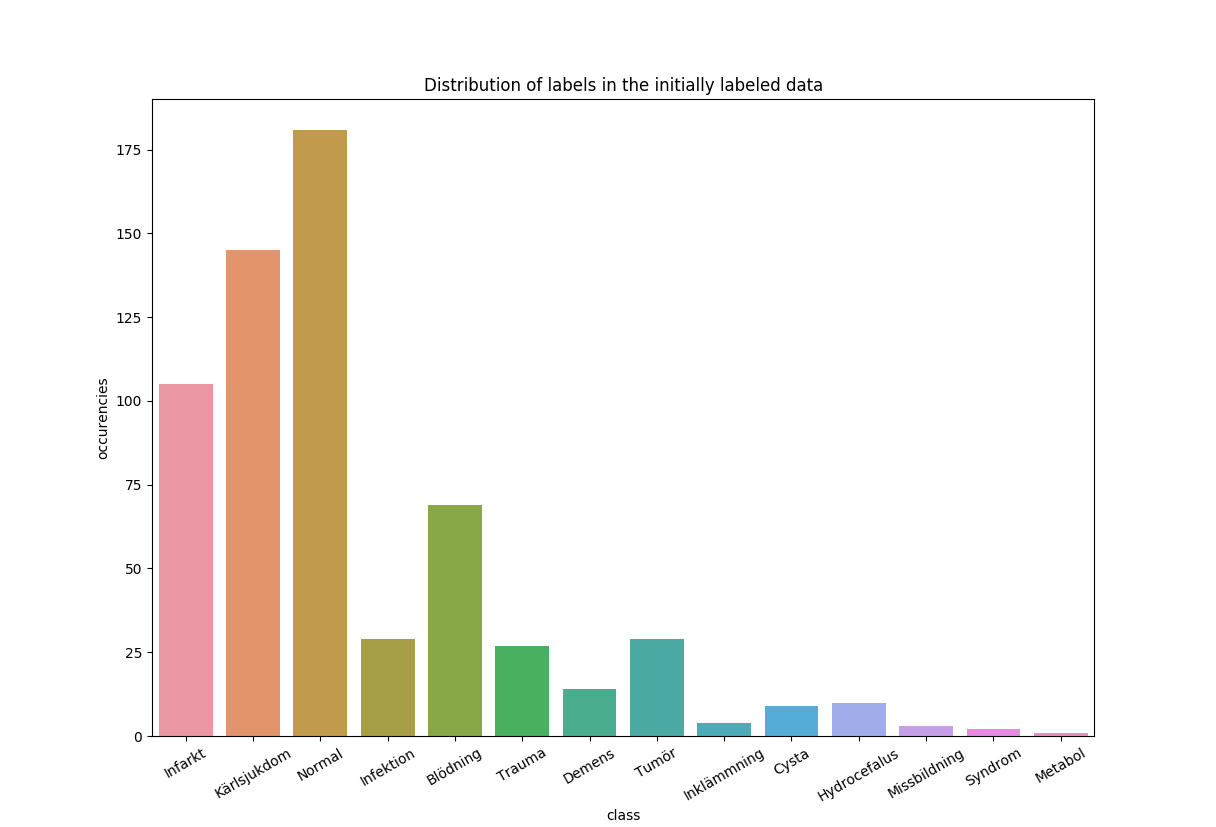
\includegraphics[width=\textwidth]{figures/class-distribution.png}
    \caption{The distribution over the labels in the initial set of labeled data provided by Sectra}
    \label{fig:class-distribution}
\end{figure}

The Reuters-21578 newswire dataset is widely used when it comes to text classification research, and provides a good multi-label benchmark that can be used to compare how well certain techniques perform to other papers.
All experiments used the \textit{ModApte} split of the dataset, which is commonly used and readily available. %TODO: Footnote with the dataset?
It splits the dataset into a predefined set of training and test documents, containing 7.769 and 3.019 entries respectively.
This split contains a subset of the categories, specifically 90 different ones.
Since the clinical dataset from Sectra only contained 15 different categories, this would not mirror that very well, so instead the 15 most common categories of those were taken out.
The distribution of the top 15 Reuters-21578 categories can be seen in Figure~\ref{fig:class-distribution-reuters}.
After filtering out the documents not labeled with any of the top 15 categories, there were 6880 documents left in the training set, and 2646 in the test set.

\begin{figure}
    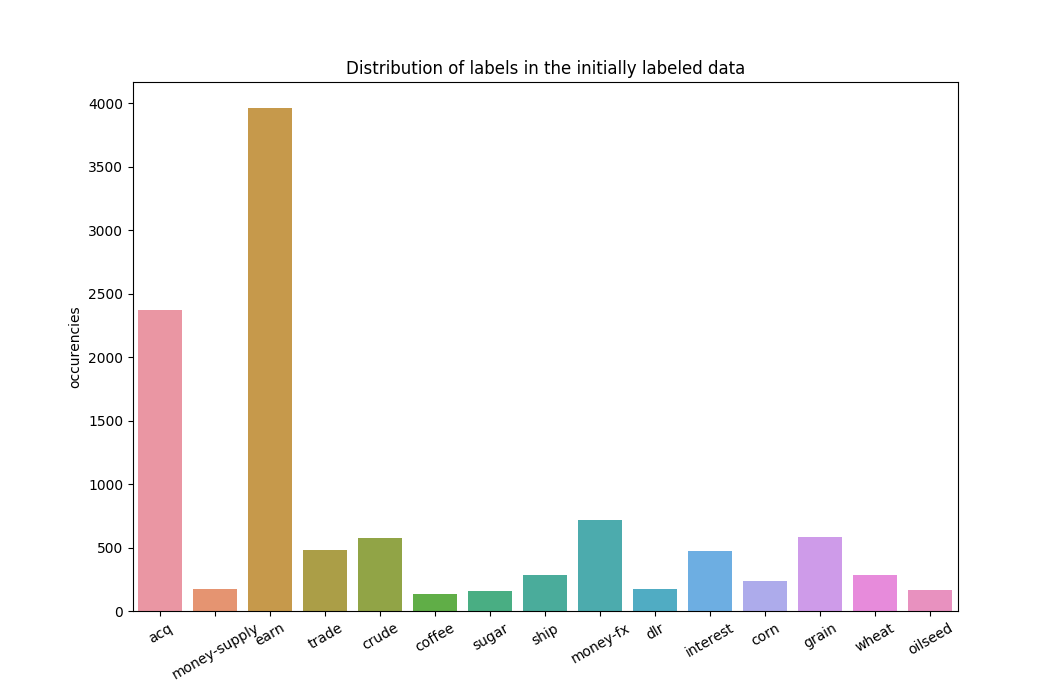
\includegraphics[width=\textwidth]{figures/class-distribution-reuters.png}
    \caption{The distribution over the labels in the Reuters data}
    \label{fig:class-distribution-reuters}
\end{figure}

\section{Pre-Processing and Text Representation}\label{sec:pre-processing}

Before the data was used in the experiments, several pre-processing steps were applied in order to clean the dataset and make it easier to work with.
The steps were:
\begin{enumerate}
    \item The first step was to extract the fields of interest.
          For the exploratory phase, and for the use of active learning techniques these were ``ReportText'' and ``Anamnesis''.
          When it came to filter out invalid reports, the ``ReportText'' was the only field of concern.
          It describes the results of the examination, and therefore if there was an examination at all.
    \item White space and punctuation were stripped from the data.
    \item All words were transformed into lowercase.
    \item The most common words as well as very infrequent words were both filtered out.
          Specifically, words occurring in less than 1\% of the documents, and words occurring in more than 90\% were removed.
          The idea behind this is that these words would not contribute to differentiating different classes of documents.
          Removing of both frequent and infrequent words is commonly done when working with text and has been done in the context of classification, active learning or topic modeling before~\cite{tong2001support, blei2003latent, brinker2006active, sarioglu2013topic}.
    \item A list of identified common stopwords were removed as well.
          Stopwords are words that are not deemed to be of significance.
          This list of words was based on the Swedish nltk stopwords list.
          After iterating over the dataset words that occurred frequently but were not considered to be very informative for the models were identified.
          The list of stopwords was then extended to incorporate these words as dataset-specific information.
          For example, this included names of the doctors that had written the report.
          By removing names of doctors the idea is to make the system more applicable to new reports, written by other doctors.
    \item Accents from the words were removed.
    \item The text was tokenized and then stemmed using the Swedish Porter2 stemmer \footnote{Swedish Porter Stemmer, http://snowball.tartarus.org/algorithms/swedish/stemmer.html}.
          Stemming is the task of making words of different plurality and tense into a common base form.
\end{enumerate}
Most of these steps have been performed in previous research  dealing with text analysis in the form of classification or active learning~\cite{tong2001support, blei2003latent, brinker2006active, sarioglu2013topic}.

After transforming the text into a sequence of tokens, the final step before using it with the models was to create a representation that would be beneficial to work with.
The representation chosen was bag of words, i.e. a matrix of tokens count.
Each document is represented by the counts of each token, disregarding the order of the tokens.
In order to get some positional information into the representation additional tokens are stored. 
The additional tokens are bigrams, which are pairs of tokens (i.e. processed words).
By storing the frequency of how often such a pair occurs in the document, alongside the regular one word tokens, some positional information is retained.

\section{Exploratory Study}\label{sec:exploratory-study}
For the exploratory study we used the representation described in Section~\ref{sec:pre-processing}.
The main goal of this phase was to get to know and to better understand the dataset.
A part of this goal was to go through the fields for the different reports to see how they worked and what values could be expected.
In order to visualize the data in a 2D plot, t-distributed stochastic neighbor embedding (t-SNE) was used.
It is a dimensionality reduction technique, that is able to transform high dimensional data into two dimensions, while working to retain as much variance as possible.

The first step was to fit an LDA model to the data.
For the purpose of exploring the data, the number of topics was chosen to be a 100, with the hope of it not resulting in too granular topics that would be hard to manually analyze.
A 100 topics is what is in the middle of the range Chang et al\@.~\cite{chang2009reading} used for evaluating the interpretability of topics.
Since the purpose of this is only to explore the data, it seemed like a sufficient starting point.
The data points were plotted in a 2D plot after reducing the dimensions using t-SNE.
Each data point was colored based on some trait that the specific data point had.
For the exploratory study, the topic with the highest probability for a given data point was used to determine the color.
A plot of this can be seen in Figure~\ref{fig:lda-dist}.
Although it might be hard to interpret as a 2D plot in this report, the bokeh library allowed for the generation an interactive plot.
Hovering over each data point would show the content of the report and the topics assigned to it, making it a convenient way to explore the data and the generated topics.

\begin{figure}
    \centering
    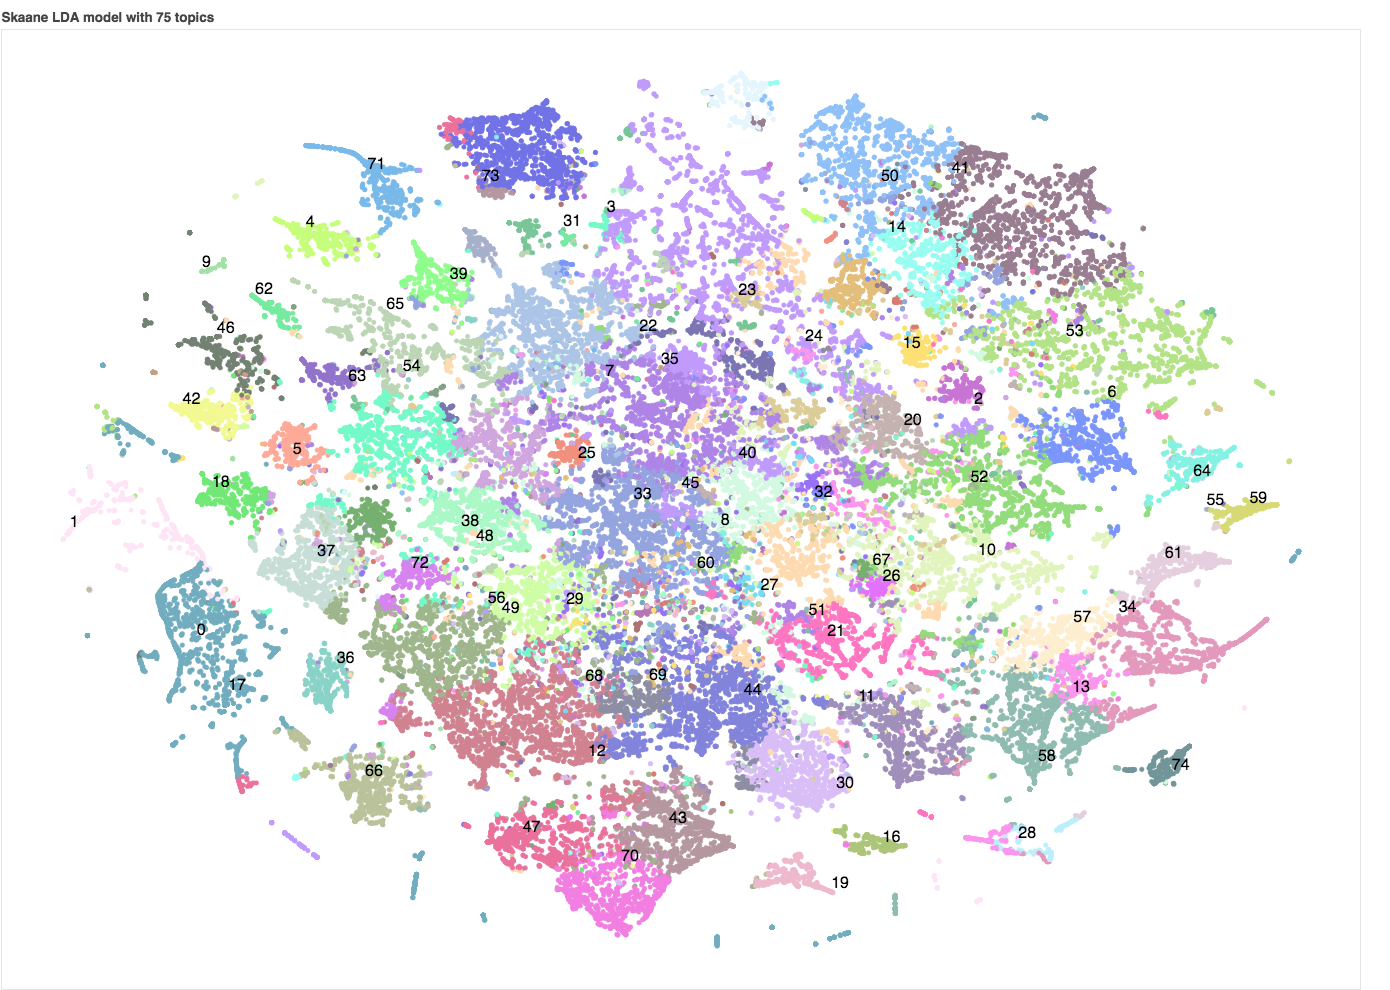
\includegraphics[width=\textwidth]{figures/lda-2d-distribution.png}
    \caption{A 2D plot of the text data, where each point is colored by topic with the highest probability}
    \label{fig:lda-dist}
\end{figure}

Samples of the generated topics can be seen in Figure~\ref{fig:topic-wordclouds}.
Another way to visualize the topics for inspection is using the techniques described by Sievert et al\@.~\cite{sievert2014ldavis}.
They propose a \textit{relevance} measure where the probability for a certain term within a topic is weighted against how common that topic is in the entire corpus.
The interactive interface provided by pyLDAvis can be seen in Figure~\ref{fig:ldavis-sample}.

\begin{figure}
    \centering
    \thirdsubfigimg{wordcloud-1}{A wordcloud over the words occurring in topic 1 for an 75 topic LDA model.}
    \thirdsubfigimg{wordcloud-17}{A wordcloud over the words occurring in topic 17 for an 75 topic LDA model}
    \caption{Wordclouds for a 75 topic LDA model}
    \label{fig:topic-wordclouds}
\end{figure}

A word2vec model was used on the entire dataset to evaluate see the relationship between terms and find possible synonyms.
In order to find synonyms, all words in the dataset that had a similarity over 95\% were manually inspected.
In addition to finding synonyms, this model was used to identify names and other identifiers in the reports.
They would come up as similar entities by the model, since they are often use in the same context.
Accomplishing this was done by exploring the data through an interactive plot, after using t-SNE to reduce the number of dimensions.

\begin{figure}
    \centering
    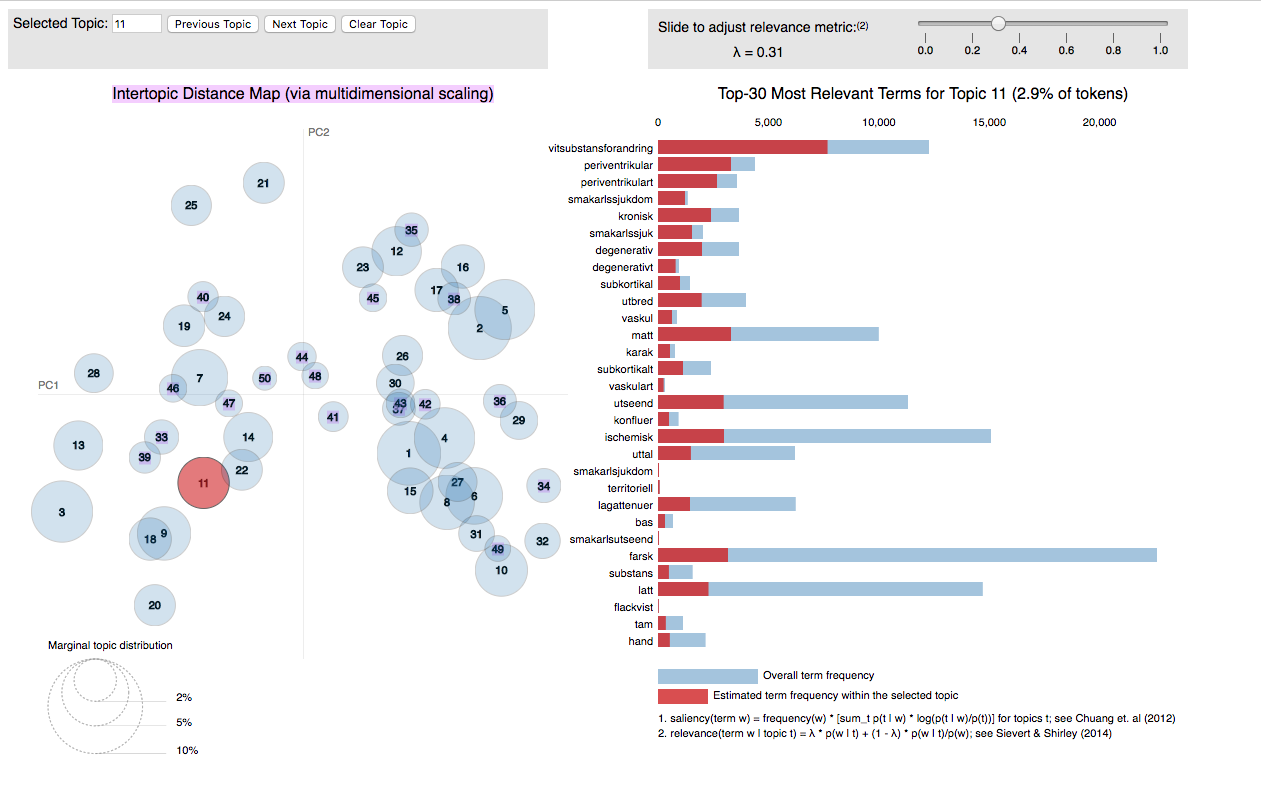
\includegraphics[width=\textwidth]{figures/ldavis-sample.png}
    \caption{A way to visualize and analyze topics based on their relevance and frequency}
    \label{fig:ldavis-sample}
\end{figure}

\section{Experiments}\label{sec:exp1-method}
In this section the experiments used to answer the research questions are described.
There is one experiment designed for each question.
The first experiment is trying to identify reports that are deemed to be invalid, the second one is a study to see what the alternatives to labeling data points at random are, as well as a comparison of how well they perform according to certain metrics.
Finally, the third one aims to compare how the distribution of labels in the labeled dataset compared between the different methods.

\subsection{Filter Out Invalid Clinical Reports Using Topic Models}




\subsection{Alternatives to Label Reports at Random}\label{sec:exp2-method}

At first, the labeled data was transformed using the LDA and k-means models.

Based on multi-label nature of the data and the results of this analysis, active learning approaches were researched with the goal of identifying methods that would be applicable in a multi-label setting.
The research touched upon both methods that exploit the structure of the data, and methods that are purely uncertainty based.

After establishing the techniques that had some indication on providing a better labeling process than sampling documents at random, they were evaluated.
In the end, the algorithms described in Section~\ref{sec:active-learning} were the ones selected for evaluation.
Some motivation for the choices are presented in Chapter~\ref{cha:results}.

The result of the simulation was used to compare the different strategies with regard to some evaluation metrics.


